%!TEX root =  cl2-lda.tex

\subsubsection{Data}

We used the annotated October 3rd 2013 presidential debate and the annonated presidential debate corpus (both obtained through Philip Resnik).
Together, the corpora are approximately 12,000 lines long.
Each line is comprised of a statement and metadata about that statement (speaker, tone, topic, etc...).
We had to preprocess the corpora, first by tokenizing it into turns in each debate, and second by performing normal preprocessing steps (e.g., tokenizing into words and removing stopwords).

In addition to the corpora, we also used the reaction data from ReactLabs (also provided by Philip Resnik).
This dataset contained 193,287 reactions by ReactLabs app \emph{users} to the October 3rd presidential debate.
Each line in the file corresponded to a single reaction (Romney:Disagree, Obama:Spin, etc...) with a timestamp and metadata about the user who submitted the reaction.

The reactions started a half hour before the debate and continued for a half hour after the debate -- we discard reactions from these time periods -- and over all the reactions are tightly clustered in time; see Fig.~\ref{fig:reactionseachturn}

\begin{figure}[]
	\centering
	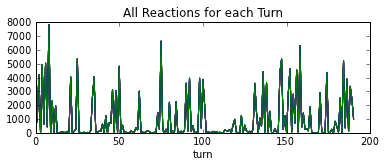
\includegraphics[scale=0.6]{Figures/reactions_for_each_turn.png}
	\caption{Reactions by all users for each turn.}
	\label{fig:reactionseachturn}
\end{figure}

The annotated debate corpus and reactions data set are synchronized allowing us to associate reactions to each \emph{turn} taken by a candidate during the debate.  However, it is common for users to react to someone who is not speaking.  In Fig.~\ref{fig:reacts_while_others_talk} we see that it is especially common for users to react to the moderator while one of the candidates is speaking, perhaps because the moderator speaks for shorter periods of time than the candidates.  Also an even larger number of reactions to the candidates are assigned to one another or the moderator, perhaps because the users are still reacting to a candidate's last turn.

\begin{figure}[]
	\centering
	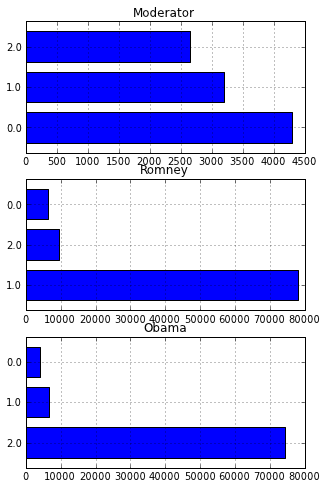
\includegraphics[scale=0.5]{Figures/reactions_while_others_are_talking}
	\caption{Reactions to the moderator (top), Romney (middle) or Obama (bottom) while speaker 0 (Moderator), 1 (Romney) or 2 (Obama) was talking.}
	\label{fig:reacts_while_others_talk}
\end{figure}

For this reason, we limit the reactions we consider to those where the reaction is associated with the person \emph{currently speaking}.  This reduces the 	number of reactions records by approximately 21\%.

Over all, we see in Fig.~\ref{fig:kinds_of_reactions_to_speakers} that reactions to Obama are overwhelmingly agreement, while a high percentage of reactions to Romney are dodge, spin or disagree reactions.

\begin{figure}[]
	\centering
	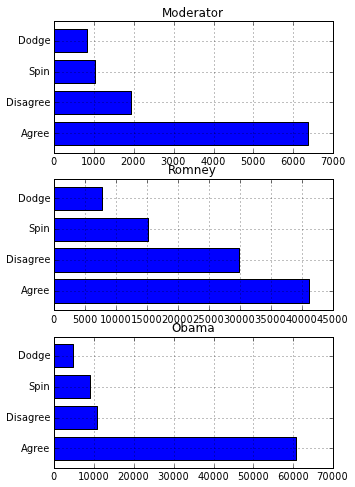
\includegraphics[scale=0.5]{Figures/kinds_of_reactions_to_speakers}
	\caption{Frequencies of reactions of each type over the course of the debate for the moderator (top), Romney (middle) and Obama (bottom).}
	\label{fig:kinds_of_reactions_to_speakers}
\end{figure}

However, this is not surprising, given the stated preferences of the users at the beginning of the debate, cf. Fig.~\ref{fig:preferred_candidates}; the users prefer Obama over Romney by over two to one.  We will see that this imbalance may create issues of bias in training examples once we begin to predict reactions of Obama or Romney supporters for what is being said in each turn.

\begin{figure}[]
	\centering
	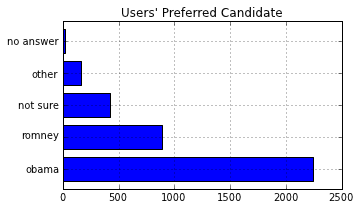
\includegraphics[scale=0.5]{Figures/preferred_candidates}
	\caption{Frequencies of each candidate as preferred by the users reacting to the debate.}
	\label{fig:preferred_candidates}
\end{figure}


\subsubsection{Resources}

We used the Machine Learning for Language Toolkit (Mallet) for several tasks in the project.
First, we used it to infer topics from the debate corpus.
Second, we used it to train several different classifiers (Decision Tree, MaxEnt, Naive Bayes).

We also used several Python modules for various jobs.
We used the natural language toolkit (NLTK) for preprocessing tasks (e.g., sentence and word tokenization, removing stopwords, etc...).
We used NumPy, SciPy, matplotlib, and Pandas for data analysis.
Finally, we used sqlite3 to store the reactions data in a format that is easier to filter.
